\documentclass[12pt,a4paper]{scrartcl}
\usepackage[T1]{fontenc}
\usepackage[utf8]{inputenc}

\usepackage{tgpagella}
\usepackage{tgadventor}
\usepackage{inconsolata}
\usepackage{tikz}
\usepackage{graphicx}
\usepackage{float}
\usepackage{minted}
\usepackage{pythontex}

\usepackage{hyperref}

\title{Using PythonTeX on Overleaf}
\author{Lian Tze Lim}
\date{}

\begin{document}

\maketitle

You need the \texttt{pythontex} package, and you need a custom \texttt{latexmkrc} file, e.g.~from \url{http://mirror.unl.edu/ctan/support/latexmk/example_rcfiles/pythontex-latexmkrc}.

Examples below are taken from \url{https://tug.org/tug2013/slides/Mertz-A_Gentle_Introduction_to_PythonTeX.pdf}

\begin{minted}{latex}
\py{2+2}
\end{minted}

\py{2+2}


\begin{minted}{latex}
Did you know that $2^{65} = \py{2**65}$?
\end{minted}

Did you know that $2^{65} = \py{2**65}$?


\begin{minted}{latex}
\begin{pycode}
lo, hi = 1, 6
print(r"\begin{tabular}{c|c}")
print(r"$m$ & $2^m$ \\ \hline")
for m in range(lo, hi + 1):
    print(r"%d & %d \\" % (m, 2**m))
print(r"\end{tabular}")
\end{pycode}
\end{minted}


\begin{pycode}
lo, hi = 1, 6
print(r"\begin{tabular}{c|c}")
print(r"$m$ & $2^m$ \\ \hline")
for m in range(lo, hi + 1):
    print(r"%d & %d \\" % (m, 2**m))
print(r"\end{tabular}")
\end{pycode}
\subsection*{Plot average monthly TMAX}
\begin{pyblock}[plot]
import numpy as np
import matplotlib.pyplot as plt
from mpl_toolkits.mplot3d import Axes3D

fig = plt.figure()
ax = Axes3D(fig)
X = np.arange(-4, 4, 0.25)
Y = np.arange(-4, 4, 0.25)
X, Y = np.meshgrid(X, Y)
R = np.sqrt(X ** 2 + Y ** 2)
Z = np.sin(R)

ax.plot_surface(X, Y, Z, rstride=1, cstride=1, cmap=plt.cm.hot)
ax.contourf(X, Y, Z, zdir='z', offset=-2, cmap=plt.cm.hot)
ax.set_zlim(-2, 2)
plt.show()
plt.savefig('discontinua-new.png')
\end{pyblock}
\begin{figure}[H]
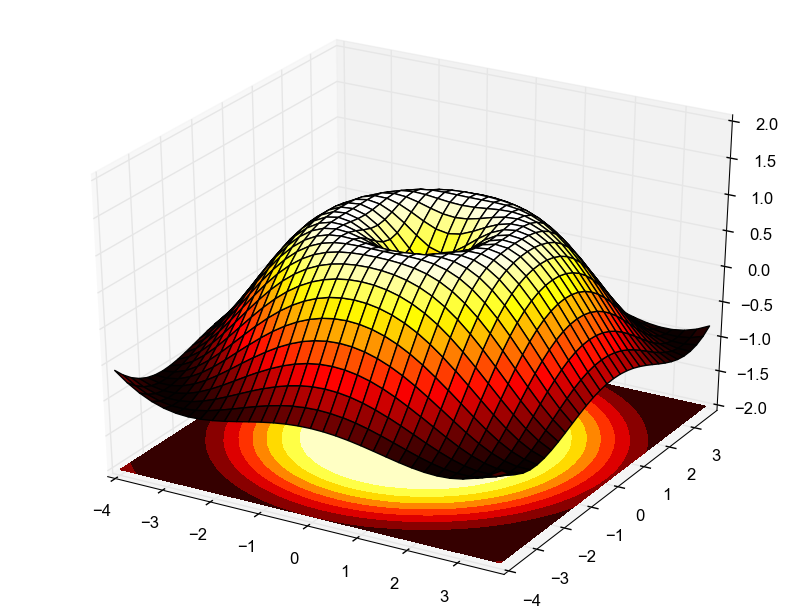
\includegraphics[scale=0.5]{figure_1.png} 
\end{figure}
\end{document}